\documentclass[10pt]{beamer}
\usetheme[progressbar=frametitle]{metropolis}
\usepackage{appendixnumberbeamer}
\usepackage{booktabs}
\usepackage[scale=2]{ccicons}
\usepackage{pgfplots}
\usepgfplotslibrary{dateplot}
\usepackage{xspace}
\usepackage{amsmath}
\usepackage{amsfonts}
\usepackage{graphicx}
\newcommand{\themename}{\textbf{\textsc{metropolis}}\xspace}
\usepackage{hyperref}

\title{LLM-as-a-Judge Reliability}
\subtitle{Phase 4 Combined Presentation}
\date{}
\author{Parsa Gholami, Aria Alyasin, Mohsen Shirazi}
\institute{Sharif University of Technology}

\begin{document}

\maketitle

\section{Category 2: Bias Quantification \& Fairness Analysis}

\begin{frame}[standout]
  \hypertarget{paper3}{}
  \Large Paper 3:\\AN EMPIRICAL ANALYSIS OF UNCERTAINTY IN LARGE LANGUAGE MODEL EVALUATIONS
\end{frame}

\begin{frame}{Category Alignment \& Positioning}
  \framesubtitle{Positioning in the Four-Pillar Taxonomy}
  \begin{itemize}
    \item \textbf{Taxonomy Alignment:} Category 2 (Bias Quantification \& Fairness Analysis)
    \item \textbf{Beyond Static Prejudices:} While prior literature focuses heavily on static evaluator biases (e.g., length, position, and brand preference), this work explores \textbf{dynamic stability}.
    \item \textbf{Internal States:} Shifting focus from verbalized outputs to internal logit probability distributions of the evaluator.
    \item \textbf{Systemic Failure:} Demonstrating how hidden evaluator uncertainty leads to fragile, non-reproducible model rankings.
  \end{itemize}
\end{frame}

\begin{frame}{Paper Overview \& Core Goals}
  \framesubtitle{An Empirical Analysis of Uncertainty in LLM-as-a-Judge}
  \begin{itemize}
    \item \textbf{The Core Problem:} Automated LLM judges are widely used to replace human raters, yet their internal evaluation confidence remains unquantified and volatile.
    \item \textbf{The Dual-Uncertainty Paradigm:} Real-world evaluations depend on a complex interaction between the judge's certainty and the candidate's generation certainty.
    \item \textbf{Three-Step Research Agenda:}
      \begin{enumerate}
        \item \textbf{Existence:} Measuring raw logit probabilities to prove uncertainty exists across major model families.
        \item \textbf{Mitigation:} Testing prompt formatting styles to stabilize decision boundaries.
        \item \textbf{Utilization:} Training an uncertainty-aware judge to spot hallucinations in out-of-distribution (OOD) scenarios.
      \end{enumerate}
  \end{itemize}
\end{frame}

% TODO SCREENSHOT: [Extract Figure 1 from the paper emperical_2.pdf showing the Raccoon trait example and save it as images/1/raccoon_concept.png]
\begin{frame}{The Dual-Uncertainty Interaction}
  \begin{figure}
    \centering
    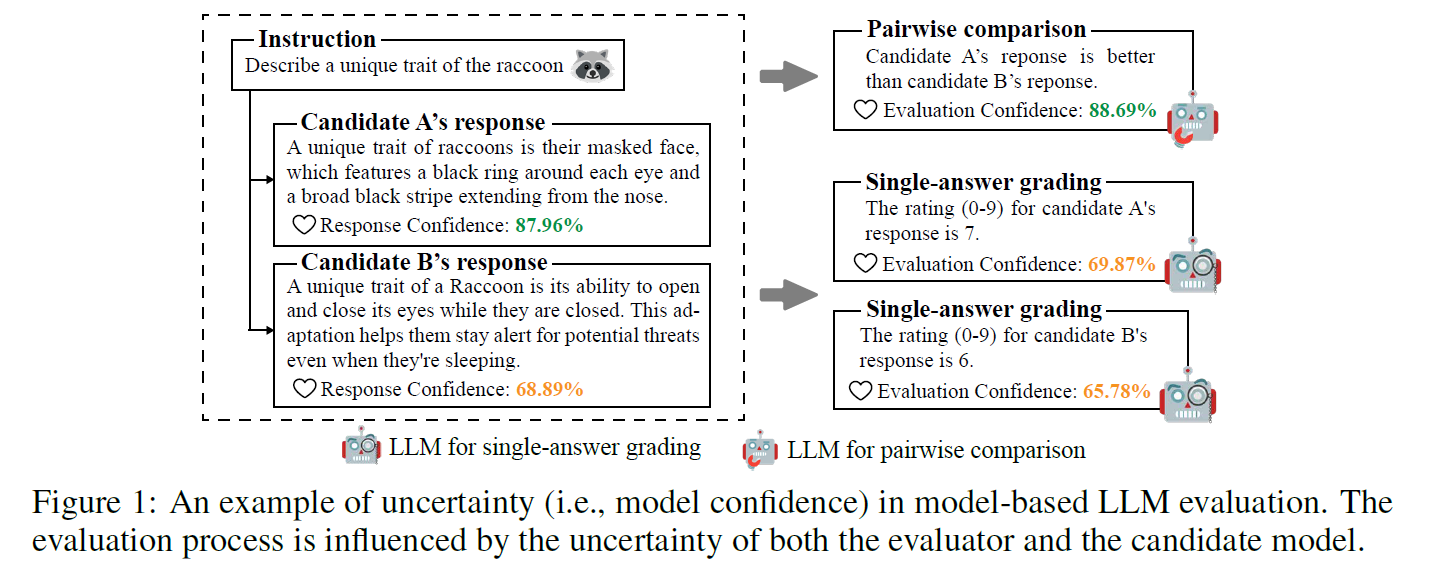
\includegraphics[width=0.9\textwidth]{images/3/raccoon_concept.png}
    \caption{Visualizing the interplay of Candidate Response Confidence and Evaluator Judge Confidence.}
  \end{figure}
\end{frame}

\begin{frame}{Part 1: Quantifying Uncertainty (Existence)}
  \framesubtitle{Deep Technical Mechanics of Logit-Based Extraction}
  \begin{itemize}
    \item \textbf{Logit-Based Probabilities:} Instead of prompting judges to verbalize confidence (which suffers from poor numeric calibration), this work extracts the raw logits directly at the last layer of generation.
    \item \textbf{Evaluation Confidence:} The precise probability of the specific token representing the final decision (e.g., the score "7" in absolute grading, or "1", "2", "Tie" in pairwise comparison).
    \item \textbf{Response Confidence:} Calculated as the mathematical average of the generation probabilities of all tokens in the candidate's output.
    \item \textbf{Zero-Cost Metadata:} Extracted directly during inference, bypassing the need for computationally expensive multi-sample consistency checks.
  \end{itemize}
\end{frame}

\begin{frame}{Part 2: Mitigating Uncertainty (Mitigation)}
  \framesubtitle{Prompt Restructuring and Structural Calibration}
  \begin{itemize}
    \item \textbf{Format-Induced Doubt:} Default templates prompt judges to output the score first. This forces an immediate decision under high attention entropy, dispersing the probability mass.
    \item \textbf{Chain-of-Thought (CoT) Calibration:} Forcing the judge to generate reasoning before the verdict token acts as a natural logit stabilizer, concentrating probability mass on the final score token.
    \item \textbf{Self-Generated References:} Instructing the judge to write its own reference answer first provides a solid comparative anchor, reducing rating volatility.
    \item \textbf{Post-Training Stabilization:} Specialized evaluator models (e.g., Prometheus2) trained in CoT formats display remarkably high confidence, but suffer from sensitivity to distribution shifts.
  \end{itemize}
\end{frame}

\begin{frame}{Part 3: Utilizing Uncertainty (ConfiLM)}
  \framesubtitle{Inherent Doubt as a Hallucination Detector}
  \begin{itemize}
    \item \textbf{The Ingestion Concept:} Candidate models express lower token probabilities when attempting to hallucinate facts. By feeding this uncertainty into the judge, the judge can detect errors.
    \item \textbf{The Verbalization Bridge:} LLMs struggle with continuous numerical float values in prompts. The authors map candidate logits into discrete natural language statements (e.g., "Highly confident", "Neutral", "Clearly doubtful").
    \item \textbf{ConfiLM Fine-Tuning:} Fine-tuning Llama-3-8B-Instruct on Alpaca data augmented with these verbalized confidence statements.
    \item \textbf{The Olympic 2024 Dataset:} A manually curated, 220-instance out-of-distribution (OOD) testing suite annotated by PhD-level experts (97.27\% agreement) to evaluate real-time factual robustness.
  \end{itemize}
\end{frame}

\begin{frame}{Part 3: Utilizing Uncertainty (ConfiLM)}
  \framesubtitle{Inherent Doubt as a Hallucination Detector}
  \begin{itemize}
    \item \textbf{The Ingestion Concept:} Candidate models express lower token probabilities when attempting to hallucinate facts. By feeding this uncertainty into the judge, the judge can detect errors.
    \item \textbf{The Verbalization Bridge:} LLMs struggle with continuous numerical float values in prompts. The authors map candidate logits into discrete natural language statements (e.g., "Highly confident", "Neutral", "Clearly doubtful").
    \item \textbf{Confidence Buckets:} Ten evenly-spaced ranges from [0.0, 0.1) $\rightarrow$ \textit{"Complete doubt"} up to [0.9, 1.0] $\rightarrow$ \textit{"Absolute confidence"}, with \textit{"Neutral"} at the midpoint [0.5, 0.6).
    \item \textbf{ConfiLM Fine-Tuning:} Fine-tuning Llama-3-8B-Instruct on Alpaca data augmented with these verbalized confidence statements.
    \item \textbf{The Olympic 2024 Dataset:} A manually curated, 220-instance out-of-distribution (OOD) testing suite annotated by PhD-level experts (97.27\% agreement) to evaluate real-time factual robustness.
  \end{itemize}
\end{frame}

% TODO SCREENSHOT: [Extract Figure 2 from the paper emperical_2.pdf showing the research pipeline diagram and save it as images/1/pipeline.png]
\begin{frame}{Multi-Phase Experimental Pipeline}
  \begin{figure}
    \centering
    
\includegraphics[width=0.9\textwidth]{images/3/pipeline.png}
    \caption{The three sequential experimental phases: Existence, Mitigation, and Utilization.}
  \end{figure}
\end{frame}

\begin{frame}{Key Empirical Findings}
  \framesubtitle{Consolidated Behavioral Observations}
  \begin{itemize}
    \item \textbf{Single-Answer vs. Pairwise Gap:} Absolute grading forces judges to evaluate in isolation, leading to high internal doubt. Pairwise comparisons provide relative anchors, resulting in highly decisive and confident assessments.
    \item \textbf{Self-Preference Bias:} Evaluations within the same model family (e.g., Llama assessing Llama) result in artificially inflated ratings paired with unwarranted confidence spikes due to shared pre-training and stylistic overlap.
    \item \textbf{The Capability Paradox:} General capability on reasoning benchmarks does not prevent evaluation doubt. Highly capable models like GPT-4o exhibit high uncertainty in default grading formats compared to less advanced models.
  \end{itemize}
\end{frame}

\begin{frame}{ConfiLM OOD Performance}
  \framesubtitle{Spotting Subtle Hallucinations in Writing Tasks}
  \begin{itemize}
    \item \textbf{OOD Challenges:} Standard judges fail in highly specific OOD domains (like real-time sports results) because they rely on in-distribution training data and overlook factual inaccuracies.
    \item \textbf{The "Rugby Sevens" Case Study:} When a candidate model generated a news report with a fabricated date, GPT-4o and standard fine-tuned models chose the hallucinated, verbose response.
    \item \textbf{The ConfiLM Victory:} By ingesting the verbalized low-confidence of the candidate, ConfiLM correctly flagged the response as inaccurate and penalized the hallucination.
  \end{itemize}
\end{frame}

\begin{frame}{Core Framework Strengths}
  \begin{itemize}
    \item \textbf{Dual-Uncertainty Interface:} Establishes the first unified framework integrating candidate generation doubt with judge decision confidence.
    \item \textbf{Zero-Cost Calibration:} Demonstrates that Chain-of-Thought (CoT) acts as a computationally free, inference-time logit stabilizer.
    \item \textbf{The Verbalization Bridge:} Successfully bypasses the numerical limits of language models by translating float values into natural adjectives.
    \item \textbf{Expert-Curated Benchmark:} The Olympic 2024 dataset provides a rigorous, highly aligned OOD testbed for automated judges.
  \end{itemize}
\end{frame}

\begin{frame}{Operational Limitations}
  \begin{itemize}
    \item \textbf{Closed-Source API Barrier:} Logit extraction is impossible on proprietary commercial platforms (such as Claude and Gemini) that withhold token probabilities.
    \item \textbf{Inference Latency Overhead:} Forcing a detailed explanation before outputting the score token elevates generation costs and runtime latency.
    \item \textbf{Exposure Bias in SFT:} Specialized judges fine-tuned on rigid templates suffer from high scoring volatility when exposed to unfamiliar domains.
  \end{itemize}
\end{frame}

\begin{frame}{Critical Strategic Outlook}
  \framesubtitle{Directions Proposed in the Paper's Discussion (\S6)}
  \begin{itemize}
    \item \textbf{Confidence-Triggered Escalation:} Future AI-evaluation platforms should establish automated confidence thresholds, triggering selective escalation to human raters for low-confidence judgments.
    \item \textbf{Multimodal Uncertainty:} Extending the framework to measure uncertainty across image, audio, and video inputs in multi-modal judges.
    \item \textbf{Multi-Turn Conversation Decay:} Investigating how evaluation uncertainty propagates or decays across complex, multi-turn dialogues.
  \end{itemize}
\end{frame}

\begin{frame}[standout]
  \hypertarget{paper5}{}
  \Large Paper 4:\\Preference Leakage: A CONTAMINATION PROBLEM IN LLM-AS-A-JUDGE
\end{frame}

\section{Introduction \& Category Alignment}

\begin{frame}{Context: The Evolution of Model Evaluation}
  \begin{itemize}
    \item \textbf{Shift in Evaluation Paradigms}:
      \begin{itemize}
        \item Traditional lexical n-gram metrics (BLEU, ROUGE) fail to capture semantic nuances in open-ended LLM outputs.
        \item \textbf{LLM-as-a-Judge} has emerged as the industry standard for scalable, fast, and human-aligned model benchmarking.
      \end{itemize}
    \vspace{0.25cm}
    \item \textbf{The Synthetic Data Engine}:
      \begin{itemize}
        \item Modern LLM alignment relies heavily on synthetic datasets generated by state-of-the-art teacher models (e.g., GPT-4o).
      \end{itemize}
    \vspace{0.25cm}
    \item \textbf{The Core Vulnerability}:
      \begin{itemize}
        \item When the model producing the training data and the model judging the student share architectural or family ties, systemic evaluation bias occurs.
      \end{itemize}
  \end{itemize}
\end{frame}

\begin{frame}{Category Alignment: Data vs. Preference Leakage}
  \begin{itemize}
    \item \textbf{Data Leakage (Classical Contamination)}:
      \begin{itemize}
        \item Direct overlap between pre-training/fine-tuning datasets and evaluation benchmark test sets.
        \item Model simply memorizes specific ground-truth questions and answers.
      \end{itemize}
    \vspace{0.35cm}
    \item \textbf{Preference Leakage (Evaluator Contamination)}:
      \begin{itemize}
        \item Structural, familial, or distillation relatedness between Data Generator ($M_G$) and Judge ($M_J$).
        \item Preferences are transferred to Student ($M_S$) via synthetic training data ($D_{syn}$).
        \item Evaluator inflates scores based on inherited stylistic and structural priors rather than objective response correctness.
      \end{itemize}
  \end{itemize}
\end{frame}

\begin{frame}{Overview Diagram: Preference vs. Data Leakage}
  % TODO SCREENSHOT: [Extract Figure 1 from the paper showing comparison between data leakage and preference leakage and save it as images/1/figure1_overview.png]
  \begin{figure}[H]
    \centering
    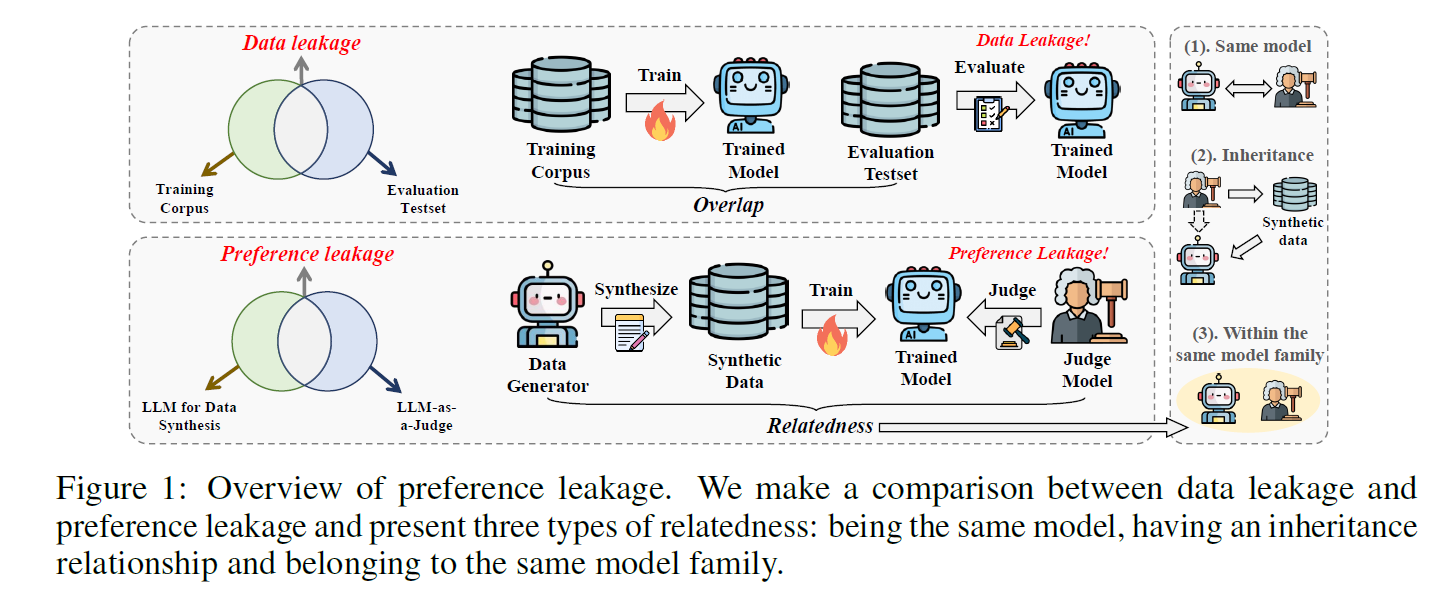
\includegraphics[width=0.85\textwidth]{images/4/figure1_overview.png}
    \caption{Conceptual Architecture of Preference Leakage and Model Lineage Relationships}
  \end{figure}
\end{frame}

% %%%%%%%%%%%%%%%%%%%%%%%%%%%%%%%%%%%%%%%%%%%%%%%%%%%%%%%%%%%%
% SECTION 2: Methodology & Detailed Pipeline
% %%%%%%%%%%%%%%%%%%%%%%%%%%%%%%%%%%%%%%%%%%%%%%%%%%%%%%%%%%%%

\section{Methodology \& Experimental Pipeline}

\begin{frame}{End-to-End Experimental Pipeline}
  \begin{itemize}
    \item \textbf{Stage 1: Seed Sampling \& Prompt Extraction}:
      \begin{itemize}
        \item Sampled 30,000 diverse open-ended prompts across diverse domains from UltraFeedback.
      \end{itemize}
    \item \textbf{Stage 2: Synthetic Data Generation ($M_G \rightarrow D_{syn}$)}:
      \begin{itemize}
        \item Teacher models ($M_G$) generate high-quality candidate responses to form instruction-tuning datasets.
      \end{itemize}
    \item \textbf{Stage 3: Student Model Post-Training ($M_S$)}:
      \begin{itemize}
        \item Base models (Mistral-7B, Qwen-2.5-14B) are trained on $D_{syn}$ via SFT, DPO, or In-Context Learning (ICL).
      \end{itemize}
    \item \textbf{Stage 4: Pairwise Evaluation \& PLS Calculation}:
      \begin{itemize}
        \item Judge models ($M_J$) evaluate $M_S$ against baseline models on Arena-Hard and AlpacaEval 2.0 to quantify score inflation.
      \end{itemize}
  \end{itemize}
\end{frame}

\begin{frame}{Part 1: Problem Definition \& Lineage Taxonomy}
  \begin{itemize}
    \item \textbf{Conceptual Formulation}:
      \begin{itemize}
        \item Evaluation score assigned by $M_J$ to $M_S$ is systematically inflated when $M_G$ is related to $M_J$.
      \end{itemize}
    \vspace{0.2cm}
    \item \textbf{Three Lineage Relatedness Categories}:
      \begin{enumerate}
        \item \textbf{Same Model}: $M_G \equiv M_J$ (e.g., GPT-4o generates synthetic training data and later evaluates the student model).
        \item \textbf{Inheritance}: $M_J$ is fine-tuned directly on $M_G$'s outputs or shares an identical fine-tuning lineage.
        \item \textbf{Same Model Family}: $M_G$ and $M_J$ share architectural design, tokenizers, and pre-training data corpora (e.g., GPT-4o and GPT-4-Turbo).
      \end{enumerate}
    \vspace{0.2cm}
    \item \textbf{Key Novelty \#1}:
      \begin{itemize}
        \item First formal taxonomy defining evaluator-generator dependency as an implicit bias channel distinct from simple self-enhancement.
      \end{itemize}
  \end{itemize}
\end{frame}

\begin{frame}{Part 2: Experimental Controls \& Metric Mechanics}
  \begin{itemize}
    \item \textbf{Controlled Experimental Setup}:
      \begin{itemize}
        \item \textbf{Data Generators / Judges}: GPT-4o, Gemini-1.5-Flash, LLaMA-3.3-70B.
        \item \textbf{Base Students}: Unaligned base models to eliminate pre-existing instruction-tuning contamination.
        \item \textbf{Benchmarks}: Arena-Hard (500 challenging prompts) and AlpacaEval 2.0 (805 prompts).
      \end{itemize}
    \vspace{0.2cm}
    \item \textbf{Preference Leakage Score (PLS) Formulation}:
      \begin{itemize}
        \item $PLS = \text{WinRate}(M_S \text{ judged by Related } M_J) - \text{WinRate}(M_S \text{ judged by Control } M_{ctrl})$.
        \item Controls for position bias (swapping model order) and length bias.
      \end{itemize}
    \vspace{0.2cm}
    \item \textbf{Key Novelty \#2}:
      \begin{itemize}
        \item A rigorous cross-evaluation benchmarking framework that isolates style inheritance from genuine reasoning quality.
      \end{itemize}
  \end{itemize}
\end{frame}

\begin{frame}{Part 3: Mechanistic Probing \& Stealth Bias}
  \begin{itemize}
    \item \textbf{The Recognition Paradox}:
      \begin{itemize}
        \item Can judges consciously detect outputs from their related student models?
        \item Direct probing reveals LLM judges perform near random chance ($30\% - 53\%$ accuracy) at identification.
      \end{itemize}
    \vspace{0.2cm}
    \item \textbf{Classifier Detectability}:
      \begin{itemize}
        \item A simple linear classifier or lightweight BERT model achieves over $82.4\%$ accuracy in identifying student generations.
      \end{itemize}
    \vspace{0.2cm}
    \item \textbf{Spurious Features as Conduits}:
      \begin{itemize}
        \item Bias is driven by surface-level artifacts: formatting templates, markdown headers, bullet-point frequency, and tone.
      \end{itemize}
    \vspace{0.2cm}
    \item \textbf{Key Novelty \#3}:
      \begin{itemize}
        \item Proving preference leakage is a subconscious phenomenon where LLM judges reward stylistic alignment without explicit awareness.
      \end{itemize}
  \end{itemize}
\end{frame}

% %%%%%%%%%%%%%%%%%%%%%%%%%%%%%%%%%%%%%%%%%%%%%%%%%%%%%%%%%%%%
% SECTION 3: Empirical Findings
% %%%%%%%%%%%%%%%%%%%%%%%%%%%%%%%%%%%%%%%%%%%%%%%%%%%%%%%%%%%%

\begin{frame}{Key Empirical Results (Verbal Summary)}
  \begin{itemize}
    \item \textbf{Widespread Score Inflation}:
      \begin{itemize}
        \item Significant positive PLS across all major model families (reaching up to $37.1\%$ win-rate inflation on Arena-Hard).
      \end{itemize}
    \vspace{0.2cm}
    \item \textbf{Model Scale Impact}:
      \begin{itemize}
        \item Smaller student models (1B--3B parameters) show \textbf{higher} leakage scores because they memorize surface-level response templates more aggressively.
      \end{itemize}
    \vspace{0.2cm}
    \item \textbf{Post-Training Method Dynamics}:
      \begin{itemize}
        \item \textbf{SFT}: Maximum leakage ($23.6\%$ average) due to heavy stylistic imitation.
        \item \textbf{DPO}: Significantly reduced leakage ($5.2\%$) by penalizing stylistic repetition.
        \item \textbf{ICL}: Minimal to zero leakage ($-2.7\%$) as core weights remain untouched.
      \end{itemize}
    \vspace{0.2cm}
    \item \textbf{Domain & Task Sensitivity}:
      \begin{itemize}
        \item Highest bias in open-ended creative writing and coding; lowest in deterministic math and logic problems.
      \end{itemize}
  \end{itemize}
\end{frame}

% %%%%%%%%%%%%%%%%%%%%%%%%%%%%%%%%%%%%%%%%%%%%%%%%%%%%%%%%%%%%
% SECTION 4: Core Framework Strengths
% %%%%%%%%%%%%%%%%%%%%%%%%%%%%%%%%%%%%%%%%%%%%%%%%%%%%%%%%%%%%

\begin{frame}{Strengths \& Methodological Rigor}
  \begin{itemize}
    \item \textbf{Pioneering Problem Formulation}:
      \begin{itemize}
        \item Uncovers a systemic vulnerability in the synthetic data lifecycle that undermines community leaderboard integrity.
      \end{itemize}
    \vspace{0.3cm}
    \item \textbf{Methodological Isolation}:
      \begin{itemize}
        \item Isolates confounding variables by starting exclusively with raw base models, avoiding instruction-tuning artifacts.
      \end{itemize}
    \vspace{0.3cm}
    \item \textbf{Broad Practical Impact}:
      \begin{itemize}
        \item Demonstrates real-world implications for major public evaluations such as LMArena, AlpacaEval, and Open LLM Leaderboard.
      \end{itemize}
  \end{itemize}
\end{frame}

% %%%%%%%%%%%%%%%%%%%%%%%%%%%%%%%%%%%%%%%%%%%%%%%%%%%%%%%%%%%%
% SECTION 5: Operational Limitations
% %%%%%%%%%%%%%%%%%%%%%%%%%%%%%%%%%%%%%%%%%%%%%%%%%%%%%%%%%%%%

\begin{frame}{Limitations \& Experimental Constraints}
  \begin{itemize}
    \item \textbf{High Computational \& API Costs}:
      \begin{itemize}
        \item Full pairwise evaluation matrices across frontier models demand massive API query volume and compute overhead.
      \end{itemize}
    \vspace{0.3cm}
    \item \textbf{Proprietary Black-Box Constraints}:
      \begin{itemize}
        \item Closed-source model providers do not disclose full pre-training data or exact model lineages, limiting complete tracking.
      \end{itemize}
    \vspace{0.3cm}
    \item \textbf{Inefficacy of Simple Prompting Mitigation}:
      \begin{itemize}
        \item Standard system prompts or Chain-of-Thought (CoT) instructions fail to remove preference leakage without structural adjustments.
      \end{itemize}
  \end{itemize}
\end{frame}

% %%%%%%%%%%%%%%%%%%%%%%%%%%%%%%%%%%%%%%%%%%%%%%%%%%%%%%%%%%%%
% SECTION 6: Strategic Outlook
% %%%%%%%%%%%%%%%%%%%%%%%%%%%%%%%%%%%%%%%%%%%%%%%%%%%%%%%%%%%%

\begin{frame}{Future Directions \& Mitigation Strategies}
  \begin{itemize}
    \item \textbf{Strict Lineage Isolation}:
      \begin{itemize}
        \item Public leaderboards must enforce strict separation between data generation teacher models and benchmark judge models.
      \end{itemize}
    \vspace{0.2cm}
    \item \textbf{Post-Hoc Statistical Calibration}:
      \begin{itemize}
        \item Use held-out human judgment samples to dynamically adjust and normalize judge scoring distributions.
      \end{itemize}
    \vspace{0.2cm}
    \item \textbf{Multi-Judge Ensembling}:
      \begin{itemize}
        \item Combine evaluations from multiple non-related model families to cancel out model-family bias.
      \end{itemize}
    \vspace{0.2cm}
    \item \textbf{Stylistic Normalization Pipelines}:
      \begin{itemize}
        \item Pre-process responses through neutralizing paraphrasers to strip surface-level formatting artifacts before judging.
      \end{itemize}
  \end{itemize}
\end{frame}

\begin{frame}{Summary \& Key Takeaways}
  \begin{itemize}
    \item \textbf{Takeaway 1}: Preference leakage is an insidious, subconscious contamination mechanism in modern LLM evaluation.
    \vspace{0.25cm}
    \item \textbf{Takeaway 2}: Judges favor student models that mirror their surface-level style, formatting, and structural cadence.
    \vspace{0.25cm}
    \item \textbf{Takeaway 3}: SFT intensifies leakage, whereas DPO, ICL, and post-hoc calibration offer effective defense pathways.
    \vspace{0.25cm}
    \item \textbf{Core Recommendation}: Decouple evaluation judges completely from synthetic training data pipelines for trustworthy benchmarks.
  \end{itemize}
\end{frame}

\end{document}
